\documentclass[11pt]{article}
\usepackage[utf8]{inputenc}
\usepackage{amsmath}
\usepackage{amsfonts}
\usepackage{amssymb}
\usepackage{graphicx}
\usepackage[super]{nth}
\usepackage{amsthm}
\usepackage{bm}
\newtheorem{theorem}{Theorem}
\newtheorem{objective}{Objective}
\newtheorem{model}{Model}
\usepackage{xcolor}
\definecolor{light-gray}{gray}{0.95}
\newcommand{\code}[1]{\colorbox{light-gray}{\texttt{#1}}}
\usepackage{listings}
\usepackage{placeins}
\usepackage{enumitem}

\usepackage[authoryear]{natbib}

\lstset{language=R}


\makeatletter
\renewcommand{\maketitle}{
\begin{center}

\pagestyle{empty}

{\Large \bf \@title\par}
\vspace{1cm}

{\LARGE Marcel Gietzmann-Sanders}\\[1cm]

STAT651 - Statistical Theory I \\
University of Alaska Fairbanks


\end{center}
}\makeatother


\title{Homework 1}

\date{2025}
\setcounter{tocdepth}{2}
\begin{document}
\maketitle

\section{Question 1}

\begin{lstlisting}
> sample( 1:10, 5, replace=TRUE )
[1] 8 2 2 1 9
\end{lstlisting}

\begin{lstlisting}
> rnorm( 5, mean=1.0, sd=0.5 )
[1] 1.909263 1.009593 1.101609 1.534538 1.542092
\end{lstlisting}


\section{Question 2}

$$I_1 = \int_0^1 x^2 dx = \frac{1}{3}x^3\Big|_0^1=\frac{1}{3}$$

$$I_2 = \int_0^1 \int_0^{2y} x dx dy = \int_0^1 \left( 0.5x^2 \Big|_0^{2y} \right)dy$$
$$= \int_0^1 2y^2 dy=\frac{2}{3}y^3 \Big|_0^1=\frac{2}{3}$$

Wolfram Alpha agrees with me on both counts. 

\begin{figure}[h!] 
	\centering
  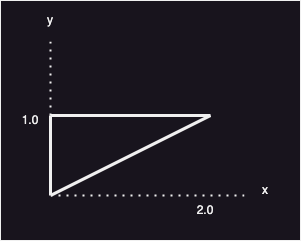
\includegraphics[height=35mm]{Sketch.png}
  \caption{Boundaries of Area Integrated in $I_2$}
  \label{fig:sketch}
\end{figure}

\FloatBarrier

\section{Question 3}

\begin{enumerate}[label=\alph*]
\item Finite - $2^4=16$ outcomes. HHHH, THHH, HTHH, TTHH, HHTH, THTH, HTTH, TTTH, HHHT, THHT, HTHT, TTHT, HHTT, THTT, HTTT, TTTT
\item Finite - 4 Heads, 3 Heads 1 Tail, 2 Heads 2 Tails, 1 Head 3 Tails, 4 Tails
\item Countably Infinite - the set I'd choose is the positive integers. While I'm sure there is a maximum number of leaves over 2" in the universe right now, life finds a way and could create a plant with more leaves over 2". 
\item Finite - I'm going to assume that lifetime here means lifetime while in use with a specific load. Given a AAA battery has a finite amount of built up charge, even assuming we can use all of it 100\% efficiently that'll give us some finite time of use under load. Let's call that value (in hours) $M$ for the lifetime of an ideal AAA (100\% efficient) battery. Our set then is [0, 1, ..., $M$] and is therefore finite. 
\item Uncountably Infinite - We're working with real numbers now so this will be a set of reals that has some range (from a small but positive value as foals can't be flat to some reasonable upper limit).
\item Finite - $S=\{ x/50 \forall x \in [0, 1, 2, ..., 50] \}$
\end{enumerate}



\end{document}